% ============================================================
%  INFORME TÉCNICO -- LABORATORIO 2: APLICACIÓN MÓVIL
%  Universidad de las Fuerzas Armadas ESPE
%  Desarrollo de Aplicaciones Móviles -- NRC 30738
% ============================================================
\documentclass[12pt,a4paper]{article}

% --- Codificación y lengua --------------------------------
\usepackage[utf8]{inputenc}
\usepackage[T1]{fontenc}
\usepackage[spanish,es-noindentfirst,es-noquoting]{babel}

% --- Márgenes ------------------------------------------
\usepackage{geometry}
\geometry{top=2.5cm, bottom=2.5cm, left=3cm, right=2.5cm}

% --- Tipografía y espaciado ----------------------------
\usepackage{lmodern}
\usepackage{microtype}
\setlength{\emergencystretch}{3em}
\usepackage{setspace}
\setstretch{1.5}
\usepackage{parskip}
\setlength{\parindent}{0pt}

% --- Gráficos ------------------------------------------
\usepackage{graphicx}
\usepackage{float}
\newfloat{anexofloat}{H}{loax}
\floatname{anexofloat}{Anexo}
\usepackage{caption}
\usepackage{subcaption}

% --- Encabezados/pies ----------------------------------
\usepackage{fancyhdr}
\setlength{\headheight}{13.6pt}
\addtolength{\topmargin}{-1.6pt}
\pagestyle{fancy}
\fancyhf{}
\fancyhead[L]{\small\textcolor{espeblue}{ESPE -- Desarrollo de Aplicaciones Móviles}}
\fancyhead[R]{\small\textcolor{espeblue}{NRC: 30738}}
\fancyfoot[C]{\thepage}
\renewcommand{\headrulewidth}{0.4pt}

% Estilo para la portada (logo centrado, sin línea)
\fancypagestyle{portada}{%
  \fancyhf{}
  \fancyhead[C]{
\includegraphics[height=2.6cm]{espe.png}}
  \renewcommand{\headrulewidth}{0pt}
}

% --- Colores -------------------------------------------
\usepackage{xcolor}
\definecolor{espeblue}{RGB}{0,51,102}
\definecolor{codegray}{rgb}{0.5,0.5,0.5}
\definecolor{codepurple}{rgb}{0.58,0,0.82}
\definecolor{backcolour}{rgb}{0.95,0.95,0.92}
\definecolor{dartblue}{RGB}{84,176,220}

% --- Secciones -----------------------------------------
\usepackage{titlesec}
\titleformat{\section}{\large\bfseries\color{espeblue}}{\thesection.}{0.5em}{}[\color{espeblue}\titlerule]
\titleformat{\subsection}{\normalsize\bfseries\color{espeblue!80}}{\thesubsection}{0.5em}{}
\titleformat{\subsubsection}{\normalsize\itshape\color{espeblue!70}}{\thesubsubsection}{0.5em}{}

% --- Tabla de contenidos -------------------------------
\usepackage{tocloft}
\renewcommand{\cftsecleader}{\cftdotfill{\cftdotsep}}
\renewcommand{\cftsubsecleader}{\cftdotfill{\cftdotsep}}

% --- Tablas -------------------------------------------
\usepackage{booktabs}
\usepackage{array}

% --- Matemáticas --------------------------------------
\usepackage{amsmath}

% --- TikZ para diagramas de flujo ---------------------
\usepackage{tikz}
\usetikzlibrary{shapes.geometric, shapes.misc, arrows.meta, positioning, calc}

\tikzset{
  startstop/.style={
    rounded rectangle, draw=espeblue, fill=espeblue!20,
    minimum width=3.2cm, minimum height=0.75cm,
    text centered, font=\small\bfseries
  },
  process/.style={
    rectangle, draw=espeblue, fill=blue!8,
    minimum width=4.2cm, minimum height=0.75cm,
    text centered, font=\small
  },
  decision/.style={
    diamond, draw=orange!70!black, fill=orange!15,
    aspect=3, minimum height=0.75cm,
    text centered, font=\small
  },
  io/.style={
    trapezium, trapezium left angle=70, trapezium right angle=110,
    draw=green!50!black, fill=green!12,
    minimum width=3.6cm, minimum height=0.75cm,
    text centered, font=\small
  },
  arrow/.style={thick, -Stealth, color=espeblue},
}

% --- Pseudocódigo ------------------------------------
\usepackage{algorithm}
\usepackage{algpseudocode}
\renewcommand{\listalgorithmname}{Índice de Algoritmos}
\floatname{algorithm}{Algoritmo}

% --- Código fuente Dart ------------------------------
\usepackage{listings}
\lstdefinelanguage{Dart}{
  keywords={abstract,as,assert,async,await,break,case,catch,class,const,continue,
    default,deferred,do,dynamic,else,enum,export,extends,extension,external,factory,
    false,final,finally,for,Function,get,hide,if,implements,import,in,interface,is,
    library,mixin,new,null,on,operator,part,rethrow,return,set,show,static,super,
    switch,sync,this,throw,true,try,typedef,var,void,while,with,yield},
  sensitive=true,
  morecomment=[l]{//},
  morecomment=[s]{/*}{*/},
  morestring=[b]",
  morestring=[b]',
}
\lstdefinestyle{dartStyle}{
  backgroundcolor=\color{backcolour},
  commentstyle=\color{codegray}\itshape,
  keywordstyle=\color{espeblue}\bfseries,
  numberstyle=\tiny\color{codegray},
  stringstyle=\color{codepurple},
  basicstyle=\ttfamily\footnotesize,
  breaklines=true,
  captionpos=b,
  numbers=left,
  numbersep=5pt,
  tabsize=2,
  frame=single,
  rulecolor=\color{espeblue!40},
}
\lstset{style=dartStyle, language=Dart}

% --- Hipervínculos ------------------------------------
\usepackage{hyperref}
\hypersetup{
  colorlinks=true,
  linkcolor=espeblue,
  citecolor=espeblue,
  urlcolor=dartblue,
  pdftitle={Laboratorio 2 - Aplicación Móvil - ESPE},
}

% ============================================================
\begin{document}
% ============================================================

% ============================================================
%  PORTADA
% ============================================================
\thispagestyle{portada}
\singlespacing
\setlength{\parskip}{0pt}
\vspace*{1.2cm}
\begin{center}
  {\Large\bfseries\color{espeblue}
    UNIVERSIDAD DE LAS FUERZAS ARMADAS ESPE\\[0.3cm]}
  {\large\color{espeblue}
    Departamento de Ciencias de la Computación\\[0.2cm]
    Asignatura: Desarrollo de Aplicaciones Móviles\\[0.2cm]
    NRC: 30738\\[0.6cm]}
  \textcolor{espeblue}{\rule{\linewidth}{1.5pt}}\\[0.4cm]
  {\LARGE\bfseries\color{espeblue}
    Informe 1.2\\[0.25cm]
    Desarrollo de una Aplicación Móvil\\[0.15cm]
    con Principios de Diseño\\[0.35cm]}
  \textcolor{espeblue}{\rule{\linewidth}{1.5pt}}\\[1.0cm]
  {\large\bfseries Integrantes:}\\[0.4cm]
  \begin{tabular}{c}
    Arroyo Alfonso\\[0.15cm]
    Cáceres Germán\\[0.15cm]
    Frías Pedro\\[0.15cm]
    Llumiquinga Ariel\\
  \end{tabular}\\[1.5cm]
  {\large\textbf{Docente:} Ing. Doris Chicaiza MSc}\\[0.35cm]
  {\large\textbf{Fecha:} 4 de mayo de 2026}\\[0.35cm]
  
  {\large\textbf{Link Entregables:}}\\[0.35cm]
  {\large\url{https://github.com/Gpcaceres/grupo-moviles-poryectos.git}}\\[0.35cm]

\end{center}

\newpage
\pagenumbering{roman}

% ============================================================
%  ÍNDICES
% ============================================================
\tableofcontents

\listoffigures

\listofalgorithms
\addcontentsline{toc}{section}{Índice de Algoritmos}

\listof{anexofloat}{Índice de Anexos}
\addcontentsline{toc}{section}{Índice de Anexos}

\newpage
\pagenumbering{arabic}
\setcounter{page}{1}

% ============================================================
%  1. INTRODUCCIÓN
% ============================================================
\section{Introducción}

El diseño de interfaces de usuario constituye uno de los pilares fundamentales en el desarrollo de aplicaciones móviles modernas. Una aplicación bien estructurada no solo debe resolver problemas de negocio, sino también ofrecer una experiencia visual coherente, intuitiva y estéticamente agradable para el usuario final.

El presente documento es el informe técnico del \textbf{Laboratorio 2 -- Desarrollo de una Aplicación Móvil con Principios de Diseño}, desarrollado en la asignatura \textit{Desarrollo de Aplicaciones Móviles} de la Universidad de las Fuerzas Armadas ESPE. La aplicación, denominada \textbf{Laboratorio 2}, fue construida con el \textit{framework} \textbf{Flutter} y el lenguaje \textbf{Dart}, integrando el patrón arquitectónico \textbf{Modelo--Vista--Controlador (MVC)} con los principios del \textbf{Diseño Atómico} para estructurar los componentes de interfaz en jerarquías reutilizables.

La solución incluye: una pantalla de bienvenida animada (\textit{splash screen}), un menú principal con navegación por rutas nombradas y cinco ejercicios prácticos de cálculo.

\subsection{Objetivos}

\subsubsection{Objetivo General}

Desarrollar una aplicación móvil multiplataforma con Flutter/Dart que aplique principios de diseño de interfaz (Diseño Atómico), el patrón MVC y navegación con rutas nombradas, para resolver cinco problemas de cálculo con lógica de negocio diferenciada.

\subsubsection{Objetivos Específicos}

\begin{itemize}
  \item Implementar una pantalla de bienvenida (\textit{splash screen}) con animaciones de entrada (fundido y deslizamiento) que transite automáticamente al menú principal.
  \item Aplicar el patrón MVC para separar las responsabilidades de datos, lógica de negocio y presentación en cada ejercicio.
  \item Organizar la capa de presentación siguiendo el Diseño Atómico: átomos, moléculas, organismos y páginas.
  \item Implementar la navegación entre pantallas mediante el sistema de rutas nombradas de Flutter.
  \item Resolver cinco problemas de cálculo que cubran estructuras secuenciales, condicionales e iterativas.
\end{itemize}

% ============================================================
%  2. MARCO TEÓRICO
% ============================================================
\section{Marco Teórico}

\subsection{Flutter y Dart}

\textbf{Flutter} es un \textit{framework} de código abierto creado por Google para el desarrollo de aplicaciones nativas multiplataforma (iOS, Android, Web, Desktop) a partir de una única base de código. Utiliza el lenguaje Dart y un motor de renderizado propio (\textit{Skia}/\textit{Impeller}) que garantiza una apariencia visual consistente entre plataformas \cite{flutter2024}.

\textbf{Dart} es un lenguaje orientado a objetos, fuertemente tipado y compilado, con soporte para programación asíncrona mediante \texttt{async/await} y compilación \textit{Ahead-of-Time} (AOT) \cite{dart2024}. Sus características más relevantes son:

\begin{itemize}
  \item \textbf{Tipado estático con \textit{null safety}}: garantiza que las variables no puedan ser \texttt{null} salvo declaración explícita.
  \item \textbf{Compilación AOT y JIT}: AOT para producción y JIT para desarrollo (\textit{Hot Reload}).
\end{itemize}

\subsection{Splash Screen}

Un \textit{splash screen} (pantalla de bienvenida) es la primera pantalla visible al iniciar una aplicación móvil. Presenta el logotipo y la identidad visual mientras se carga el contenido inicial. En Flutter se implementa como la ruta inicial (\texttt{initialRoute: '/'}), utilizando \texttt{AnimationController} para efectos de entrada y \texttt{Future.delayed} para la transición automática al menú principal mediante \texttt{Navigator.pushReplacementNamed}.

\subsection{Patrón Arquitectónico MVC}

El patrón \textbf{Modelo--Vista--Controlador (MVC)} separa la aplicación en tres capas con responsabilidades bien definidas \cite{gamma1994}:

\begin{itemize}
  \item \textbf{Modelo}: encapsula los datos y la lógica de negocio. Es independiente de la interfaz gráfica.
  \item \textbf{Vista}: responsable únicamente de la presentación. No procesa ni almacena datos.
  \item \textbf{Controlador}: intermediario entre Modelo y Vista; recibe entradas del usuario, delega al Modelo y actualiza la Vista.
\end{itemize}

En Flutter, MVC se implementa organizando las carpetas \texttt{model/}, \texttt{view/} y \texttt{controller/} dentro de \texttt{lib/}.

\subsection{Diseño Atómico (\textit{Atomic Design})}

El \textbf{Diseño Atómico}, propuesto por Brad Frost \cite{frost2016}, organiza los componentes de interfaz en cinco niveles:

\begin{enumerate}
  \item \textbf{Átomos}: componentes mínimos e indivisibles (\texttt{TextField}, \texttt{Icon}, \texttt{Text}).
  \item \textbf{Moléculas}: combinación de átomos con una función concreta (campo de entrada con etiqueta).
  \item \textbf{Organismos}: grupos de moléculas que forman una sección completa (formulario + resultado).
  \item \textbf{Plantillas}: esqueleto de la pantalla sin contenido real.
  \item \textbf{Páginas}: instancias concretas con contenido real y navegación activa.
\end{enumerate}

En la aplicación, cada archivo de vista implementa los cuatro primeros niveles como clases privadas (prefijo \texttt{\_}) dentro del mismo archivo.

\subsection{Navegación con Rutas Nombradas}

Flutter gestiona la navegación mediante una pila (\textit{stack}) de rutas. Con rutas nombradas, se define un mapa \texttt{routes} en \texttt{MaterialApp} y se navega con:
\begin{itemize}
  \item \texttt{Navigator.pushNamed}: agrega una nueva pantalla a la pila (permite regresar con \textit{back}).
  \item \texttt{Navigator.pushReplacementNamed}: reemplaza la pantalla actual (usado en el splash para que no sea alcanzable con el botón atrás).
  \item \texttt{Navigator.pop}: elimina la pantalla actual y regresa a la anterior.
\end{itemize}

\subsection{Contraste: MVC versus Diseño Atómico}

\begin{table}[H]
\centering
\caption{Comparativa entre MVC y Diseño Atómico en el contexto de Flutter}
\label{tab:mvc_vs_atomic}
\renewcommand{\arraystretch}{1.4}
\begin{tabular}{>{\bfseries}p{3.2cm} p{5cm} p{5cm}}
\toprule
Criterio & MVC & Diseño Atómico \\
\midrule
Enfoque & Separación de capas lógicas & Composición jerárquica de UI \\
Nivel de abstracción & Arquitectura de la aplicación & Organización interna de la vista \\
Unidad base & Módulo funcional (model/controller/view) & Widget atómico \\
Reutilización & Por capa y por función & Por nivel de composición \\
Estructura en Flutter & Carpetas \texttt{model/}, \texttt{view/}, \texttt{controller/} & Átomos, moléculas y organismos dentro de cada vista \\
\bottomrule
\end{tabular}
\end{table}

Ambos paradigmas son complementarios: MVC rige la organización de archivos a nivel de carpetas, mientras que Diseño Atómico guía la composición interna de cada Vista.

% ============================================================
%  3. METODOLOGÍA
% ============================================================
\section{Metodología}

El desarrollo de la aplicación siguió un proceso iterativo e incremental:

\begin{enumerate}
  \item \textbf{Análisis de requisitos}: identificación de los cinco ejercicios, sus entradas, salidas y reglas de negocio.
  \item \textbf{Diseño del splash screen}: definición de animaciones, identidad visual y transición automática.
  \item \textbf{Diseño arquitectónico}: estructura MVC con carpetas \texttt{model/}, \texttt{view/}, \texttt{controller/}.
  \item \textbf{Modelado}: clases Dart puras con lógica de cálculo, sin dependencias de Flutter.
  \item \textbf{Implementación de controladores}: parseo y validación de entradas del usuario.
  \item \textbf{Diseño de vistas}: construcción de interfaces aplicando Diseño Atómico (átomos $\rightarrow$ moléculas $\rightarrow$ organismos $\rightarrow$ páginas).
  \item \textbf{Integración}: configuración de rutas nombradas en \texttt{main.dart} y menú principal.
  \item \textbf{Pruebas}: verificación manual en emulador Android.
\end{enumerate}

\subsection{Herramientas y Tecnologías Utilizadas}

\begin{itemize}
  \item \textbf{Flutter SDK 3.x} / \textbf{Dart 3.x}: \textit{framework} y lenguaje con \textit{null safety}.
  \item \textbf{Visual Studio Code} con extensiones Flutter y Dart.
  \item \textbf{Android Emulator}: entorno de emulación y pruebas.
  \item \textbf{Git / GitHub}: control de versiones.
\end{itemize}

\subsection{Estructura del Proyecto}

{\small
\begin{verbatim}
lib/
  main.dart                       <- Punto de entrada y rutas nombradas
  model/
    venta_model.dart              <- Factura con IVA, descuento y comisión
    banco_model.dart              <- Cuenta de ahorros compuesta mensual
    salon_model.dart              <- Promedios por salón y escuela
    caja_model.dart               <- Caja registradora por denominaciones
    ventas_analisis_model.dart    <- Análisis de ventas por categorías
  controller/
    venta_controller.dart
    banco_controller.dart
    salon_controller.dart
    caja_controller.dart
    ventas_analisis_controller.dart
  view/
    splash_view.dart              <- Pantalla de bienvenida animada
    menu_view.dart                <- Menú principal con rutas nombradas
    venta_view.dart
    banco_view.dart
    salon_view.dart
    caja_view.dart
    ventas_analisis_view.dart
\end{verbatim}
}

% ============================================================
%  4. DESARROLLO
% ============================================================
\section{Desarrollo}

\subsection{Splash Screen -- Pantalla de Bienvenida}

\subsubsection{Descripción}

La pantalla de bienvenida es la primera pantalla visible al iniciar la aplicación. Muestra el logotipo y el nombre de la aplicación sobre un fondo degradado azul, con animaciones de fundido (\textit{fade-in}) y deslizamiento (\textit{slide-up}) durante 1500\,ms. Tras 3 segundos, transita automáticamente al menú principal.

\subsubsection{Implementación con Diseño Atómico}

\begin{itemize}
  \item \textbf{Átomo} \texttt{\_SplashLogo}: icono \texttt{calculate\_rounded} sobre un círculo semitransparente.
  \item \textbf{Átomo} \texttt{\_SplashTitle}: título ``Laboratorio 2'', subtítulo y nombre del grupo.
  \item \textbf{Molécula} \texttt{\_SplashLoader}: \texttt{CircularProgressIndicator} con texto ``Cargando\ldots''.
  \item \textbf{Organismo} \texttt{\_SplashCard}: composición vertical de logo, título y loader.
  \item \begin{sloppypar}\textbf{Página} \texttt{SplashView}: \texttt{StatefulWidget} con \texttt{Animation\allowbreak{}Controller}, \texttt{FadeTransition} + \texttt{Slide\allowbreak{}Transition} y \texttt{Future.delayed(3s)} $\rightarrow$ \texttt{push\allowbreak{}ReplacementNamed('/menu')}.\end{sloppypar}
\end{itemize}

% -----------------------------------------------
\subsection{Problema 1 -- Venta y Factura}

\subsubsection{Descripción}

El vendedor ingresa una lista de productos (nombre, precio, cantidad) y su sueldo base. La aplicación calcula la factura completa: subtotal, IVA, descuento por volumen, total final y el sueldo total del vendedor incluyendo comisión.

\textbf{Reglas de negocio:}
\begin{align}
  \text{subtotal}      &= \sum_{i=1}^{n} \text{precio}_i \times \text{cantidad}_i \\[4pt]
  \text{IVA}           &= \text{subtotal} \times 0{,}15 \\[4pt]
  \text{subtotalIVA}   &= \text{subtotal} + \text{IVA} \\[4pt]
  \text{descuento}     &= \begin{cases} \text{subtotalIVA} \times 0{,}20 & \text{si subtotalIVA} > 2000 \\ 0 & \text{caso contrario} \end{cases} \\[4pt]
  \text{totalFinal}    &= \text{subtotalIVA} - \text{descuento} \\[4pt]
  \text{comisión}      &= \text{subtotal} \times 0{,}05 \\[4pt]
  \text{sueldoTotal}   &= \text{sueldoBase} + \text{comisión}
\end{align}

\subsubsection{Diagrama de Flujo}

\begin{figure}[H]
\centering
\resizebox{\linewidth}{!}{%
\begin{tikzpicture}[node distance=0.85cm]
  \node (start)   [startstop]                   {INICIO};
  \node (in1)     [io,      below=of start]     {Ingresar productos y sueldoBase};
  \node (sub)     [process, below=of in1]       {subtotal = $\sum$ precio$_i \times$ cantidad$_i$};
  \node (iva)     [process, below=of sub]       {IVA = subtotal $\times$ 0.15};
  \node (sivd)    [process, below=of iva]       {subtotalIVA = subtotal + IVA};
  \node (dec)     [decision,below=of sivd]      {subtotalIVA $>$ 2000?};
  \node (desc)    [process, below left=1.1cm and 1.8cm of dec]  {descuento = subtotalIVA $\times$ 0.20};
  \node (nodesc)  [process, below right=1.1cm and 1.8cm of dec] {descuento = 0};
  \node (total)   [process, below=2.4cm of dec] {totalFinal = subtotalIVA $-$ descuento};
  \node (com)     [process, below=of total]     {comisión = subtotal $\times$ 0.05};
  \node (sueldo)  [process, below=of com]       {sueldoTotal = sueldoBase + comisión};
  \node (out)     [io,      below=of sueldo]    {Mostrar factura y sueldo};
  \node (stop)    [startstop, below=of out]     {FIN};

  \draw [arrow] (start)  -- (in1);
  \draw [arrow] (in1)    -- (sub);
  \draw [arrow] (sub)    -- (iva);
  \draw [arrow] (iva)    -- (sivd);
  \draw [arrow] (sivd)   -- (dec);
  \draw [arrow] (dec)    -- node[above left,font=\small]{Sí} (desc);
  \draw [arrow] (dec)    -- node[above right,font=\small]{No} (nodesc);
  \draw [arrow] (desc)   |- (total);
  \draw [arrow] (nodesc) |- (total);
  \draw [arrow] (total)  -- (com);
  \draw [arrow] (com)    -- (sueldo);
  \draw [arrow] (sueldo) -- (out);
  \draw [arrow] (out)    -- (stop);
\end{tikzpicture}
}%
\caption{Diagrama de flujo -- Problema 1: Venta y Factura}
\label{fig:flujo_p1}
\end{figure}

\subsubsection{Pseudocódigo}

\begin{algorithm}[H]
\caption{Cálculo de Factura con IVA, Descuento y Comisión}
\label{alg:venta}
\begin{algorithmic}[1]
  \Require $\text{productos} = [(p_i, c_i)],\ \text{sueldoBase} \geq 0$
  \Ensure $\text{totalFinal},\ \text{sueldoTotal}$
  \State $subtotal \leftarrow \sum p_i \times c_i$
  \State $IVA \leftarrow subtotal \times 0.15$
  \State $subtotalIVA \leftarrow subtotal + IVA$
  \If{$subtotalIVA > 2000$}
    \State $descuento \leftarrow subtotalIVA \times 0.20$
  \Else
    \State $descuento \leftarrow 0$
  \EndIf
  \State $totalFinal \leftarrow subtotalIVA - descuento$
  \State $comision \leftarrow subtotal \times 0.05$
  \State $sueldoTotal \leftarrow sueldoBase + comision$
  \State \textbf{MOSTRAR} $subtotal,\ IVA,\ descuento,\ totalFinal,\ sueldoTotal$
\end{algorithmic}
\end{algorithm}

\subsubsection{Implementación MVC}

\begin{itemize}
  \item \textbf{Modelo} (\texttt{venta\_model.dart}): clases \texttt{ProductoItem} (nombre, precio, cantidad, getter \texttt{subtotal}) y \texttt{FacturaResultado} con método estático \texttt{calcular\allowbreak(List<\allowbreak{}ProductoItem>,~sueldoBase)}.
  \item \textbf{Controlador} (\texttt{venta\_controller.dart}): valida y parsea las entradas de texto del usuario, construye la lista de productos y delega al modelo.
  \item \textbf{Vista} (\texttt{venta\_view.dart}): \texttt{StatefulWidget} con AppBar azul. Lista dinámica de productos. Átomos: campos de texto. Moléculas: fila de producto. Organismo: formulario + resultados. Página: \texttt{VentaPage}.
\end{itemize}

% -----------------------------------------------
\subsection{Problema 4.9 -- Cuenta de Ahorros}

\subsubsection{Descripción}

Se deposita una cantidad fija mensual en una cuenta de ahorros con capitalización compuesta mensual a una tasa nominal anual del 10\%. La aplicación calcula el saldo acumulado al final de cada año durante $N$ años.

\textbf{Fórmula de capitalización compuesta mensual:}
\[
  r_m = \frac{0{,}10}{12}, \qquad
  S_m = (S_{m-1} + D) \times (1 + r_m)
\]

donde $D$ es el depósito mensual, $S_m$ el saldo al mes $m$ y $r_m$ la tasa mensual.

\subsubsection{Diagrama de Flujo}

\begin{figure}[H]
\centering
\begin{tikzpicture}[node distance=0.85cm]
  \node (start)   [startstop]                   {INICIO};
  \node (in1)     [io,      below=of start]     {Ingresar depósito mensual $D$ y años $N$};
  \node (init)    [process, below=of in1]       {saldo = 0,\ \ $r_m$ = 0.10 / 12};
  \node (loop1)   [process, below=of init]      {Para anio = 1 hasta $N$};
  \node (loop2)   [process, below=of loop1]     {\quad Para mes = 1 hasta 12};
  \node (calc)    [process, below=of loop2]     {\quad\quad saldo = (saldo + $D$) $\times$ (1 + $r_m$)};
  \node (endloop2)[process, below=of calc]      {\quad Fin mes};
  \node (out)     [io,      below=of endloop2]  {\quad Registrar saldo del año};
  \node (endloop1)[process, below=of out]       {Fin año};
  \node (show)    [io,      below=of endloop1]  {Mostrar tabla de saldos por año};
  \node (stop)    [startstop, below=of show]    {FIN};

  \draw [arrow] (start)    -- (in1);
  \draw [arrow] (in1)      -- (init);
  \draw [arrow] (init)     -- (loop1);
  \draw [arrow] (loop1)    -- (loop2);
  \draw [arrow] (loop2)    -- (calc);
  \draw [arrow] (calc)     -- (endloop2);
  \draw [arrow] (endloop2) -- (out);
  \draw [arrow] (out)      -- (endloop1);
  \draw [arrow] (endloop1) -- (show);
  \draw [arrow] (show)     -- (stop);
\end{tikzpicture}
\caption{Diagrama de flujo -- Problema 4.9: Cuenta de Ahorros}
\label{fig:flujo_p49}
\end{figure}

\subsubsection{Pseudocódigo}

\begin{algorithm}[H]
\caption{Saldo de Cuenta de Ahorros con Capitalización Compuesta Mensual}
\label{alg:banco}
\begin{algorithmic}[1]
  \Require $D > 0,\ N \geq 1$
  \Ensure $\text{tabla de saldos por año}$
  \State $saldo \leftarrow 0$
  \State $r_m \leftarrow 0.10 \div 12$
  \For{$anio \leftarrow 1$ \textbf{hasta} $N$}
    \For{$mes \leftarrow 1$ \textbf{hasta} $12$}
      \State $saldo \leftarrow (saldo + D) \times (1 + r_m)$
    \EndFor
    \State \textbf{REGISTRAR} $(anio,\ saldo)$
  \EndFor
  \State \textbf{MOSTRAR} tabla de resultados
\end{algorithmic}
\end{algorithm}

\subsubsection{Implementación MVC}

\begin{itemize}
  \item \textbf{Modelo} (\texttt{banco\_model.dart}): clase \texttt{BancoAnioResultado} (año, saldoFinal) y \texttt{BancoModel\allowbreak.calcular\allowbreak(depositoMensual, nAnios)} que retorna \texttt{List<\allowbreak{}BancoAnioResultado>}.
  \item \textbf{Controlador} (\texttt{banco\_controller.dart}): parsea y valida las entradas de texto y delega el cálculo al modelo.
  \item \textbf{Vista} (\texttt{banco\_view.dart}): AppBar índigo. Tabla de resultados con año y saldo formateado. \texttt{BancoPage}.
\end{itemize}

% -----------------------------------------------
\subsection{Problema 4.10 -- Promedios de Salones}

\subsubsection{Descripción}

Se tienen $S$ salones, cada uno con $n_i$ alumnos. Para cada salón se calcula el promedio de edades y finalmente se obtiene el promedio general de toda la escuela.

\textbf{Fórmulas:}
\[
  \bar{x}_i = \frac{\displaystyle\sum_{j=1}^{n_i} e_{ij}}{n_i}, \qquad
  \bar{x}_{\text{escuela}} = \frac{\displaystyle\sum_{i=1}^{S}\sum_{j=1}^{n_i} e_{ij}}{\displaystyle\sum_{i=1}^{S} n_i}
\]

\subsubsection{Diagrama de Flujo}

\begin{figure}[H]
\centering
\begin{tikzpicture}[node distance=0.85cm]
  \node (start)  [startstop]                   {INICIO};
  \node (in1)    [io,      below=of start]     {Ingresar número de salones $S$};
  \node (loop1)  [process, below=of in1]       {Para $i$ = 1 hasta $S$};
  \node (in2)    [io,      below=of loop1]     {\quad Ingresar edades del salón $i$};
  \node (avg)    [process, below=of in2]       {\quad $\bar{x}_i$ = suma$_i$ / $n_i$};
  \node (reg)    [io,      below=of avg]       {\quad Registrar ($i$, $\bar{x}_i$)};
  \node (endl)   [process, below=of reg]       {Fin salón};
  \node (esc)    [process, below=of endl]      {$\bar{x}_{esc}$ = suma total / total alumnos};
  \node (out)    [io,      below=of esc]       {Mostrar promedios y promedio escuela};
  \node (stop)   [startstop, below=of out]     {FIN};

  \draw [arrow] (start) -- (in1);
  \draw [arrow] (in1)   -- (loop1);
  \draw [arrow] (loop1) -- (in2);
  \draw [arrow] (in2)   -- (avg);
  \draw [arrow] (avg)   -- (reg);
  \draw [arrow] (reg)   -- (endl);
  \draw [arrow] (endl)  -- (esc);
  \draw [arrow] (esc)   -- (out);
  \draw [arrow] (out)   -- (stop);
\end{tikzpicture}
\caption{Diagrama de flujo -- Problema 4.10: Promedios de Salones}
\label{fig:flujo_p410}
\end{figure}

\subsubsection{Pseudocódigo}

\begin{algorithm}[H]
\caption{Cálculo de Promedios de Salones y Escuela}
\label{alg:salon}
\begin{algorithmic}[1]
  \Require $S \geq 1$, edades $e_{ij} \geq 0$
  \Ensure $\bar{x}_i$ para cada salón, $\bar{x}_{escuela}$
  \State $totalEdades \leftarrow 0$;\ $totalAlumnos \leftarrow 0$
  \For{$i \leftarrow 1$ \textbf{hasta} $S$}
    \State \textbf{LEER} $[e_{i1}, e_{i2}, \ldots, e_{in_i}]$
    \State $\bar{x}_i \leftarrow \sum e_{ij} \div n_i$
    \State \textbf{REGISTRAR} $(i,\ \bar{x}_i)$
    \State $totalEdades \leftarrow totalEdades + \sum e_{ij}$
    \State $totalAlumnos \leftarrow totalAlumnos + n_i$
  \EndFor
  \State $\bar{x}_{escuela} \leftarrow totalEdades \div totalAlumnos$
  \State \textbf{MOSTRAR} promedios por salón y $\bar{x}_{escuela}$
\end{algorithmic}
\end{algorithm}

\subsubsection{Implementación MVC}

\begin{itemize}
  \item \textbf{Modelo} (\texttt{salon\_model.dart}): clase \texttt{SalonResultado} (número, edades, promedio); \texttt{SalonModel\allowbreak.calcular\allowbreak(List<List<double>>)} y \texttt{SalonModel\allowbreak.promedioEscuela\allowbreak(List<\allowbreak{}SalonResultado>)}.
  \item \textbf{Controlador} (\texttt{salon\_controller.dart}): parseo de las edades ingresadas como texto separado por comas.
  \item \textbf{Vista} (\texttt{salon\_view.dart}): formulario en dos pasos (número de salones $\rightarrow$ edades). AppBar teal. \texttt{SalonPage}.
\end{itemize}

% -----------------------------------------------
\subsection{Problema 4.12 -- Caja Registradora}

\subsubsection{Descripción}

El cajero registra la cantidad de billetes y monedas de cada denominación en caja. La aplicación calcula el subtotal por denominación y el total general.

\textbf{Fórmula:}
\[
  \text{subtotal}_i = \text{denominación}_i \times \text{cantidad}_i, \qquad
  \text{total} = \sum_{i=1}^{n} \text{subtotal}_i
\]

\subsubsection{Diagrama de Flujo}

\begin{figure}[H]
\centering
\begin{tikzpicture}[node distance=0.85cm]
  \node (start)  [startstop]                   {INICIO};
  \node (in1)    [io,      below=of start]     {Ingresar denominaciones y cantidades};
  \node (loop)   [process, below=of in1]       {Para cada denominación $i$};
  \node (calc)   [process, below=of loop]      {\quad subtotal$_i$ = denominación$_i \times$ cantidad$_i$};
  \node (endl)   [process, below=of calc]      {Fin denominación};
  \node (total)  [process, below=of endl]      {total = $\sum$ subtotal$_i$};
  \node (out)    [io,      below=of total]     {Mostrar subtotales y total};
  \node (stop)   [startstop, below=of out]     {FIN};

  \draw [arrow] (start) -- (in1);
  \draw [arrow] (in1)   -- (loop);
  \draw [arrow] (loop)  -- (calc);
  \draw [arrow] (calc)  -- (endl);
  \draw [arrow] (endl)  -- (total);
  \draw [arrow] (total) -- (out);
  \draw [arrow] (out)   -- (stop);
\end{tikzpicture}
\caption{Diagrama de flujo -- Problema 4.12: Caja Registradora}
\label{fig:flujo_p412}
\end{figure}

\subsubsection{Pseudocódigo}

\begin{algorithm}[H]
\caption{Cálculo de Totales en Caja Registradora}
\label{alg:caja}
\begin{algorithmic}[1]
  \Require denominaciones $d_i > 0$, cantidades $c_i \geq 0$
  \Ensure subtotales por denominación y total general
  \State $total \leftarrow 0$
  \For{cada denominación $i$}
    \State $subtotal_i \leftarrow d_i \times c_i$
    \State $total \leftarrow total + subtotal_i$
  \EndFor
  \State \textbf{MOSTRAR} $subtotal_i$ para cada $i$ y $total$
\end{algorithmic}
\end{algorithm}

\subsubsection{Implementación MVC}

\begin{itemize}
  \item \textbf{Modelo} (\texttt{caja\_model.dart}): clase \texttt{BilleteMoneda} (denominación, cantidad, getter \texttt{subtotal}) y \texttt{CajaModel.calcularTotal(List<BilleteMoneda>)}.
  \item \textbf{Controlador} (\texttt{caja\_controller.dart}): construye la lista de denominaciones a partir de las cantidades ingresadas por el usuario.
  \item \textbf{Vista} (\texttt{caja\_view.dart}): tabla de denominaciones fijas con campos editables. AppBar naranja. \texttt{CajaPage}.
\end{itemize}

% -----------------------------------------------
\subsection{Problema 4.13 -- Análisis de Ventas}

\subsubsection{Descripción}

Se ingresan $N$ montos de ventas. Cada venta se clasifica en una de tres categorías según su monto. Se reporta el conteo, el subtotal y el porcentaje de cada categoría, más el total global.

\textbf{Criterio de clasificación:}
\[
  \text{categoría} = \begin{cases}
    \text{Baja}   & \text{si } \text{monto} \leq 10\,000 \\
    \text{Media}  & \text{si } 10\,000 < \text{monto} < 20\,000 \\
    \text{Alta}   & \text{si } \text{monto} \geq 20\,000
  \end{cases}
\]

\subsubsection{Diagrama de Flujo}

\begin{figure}[H]
\centering
\resizebox{\linewidth}{!}{%
\begin{tikzpicture}[node distance=0.9cm and 2cm]
  \node (start)  [startstop]                              {INICIO};
  \node (in1)    [io,       below=of start]               {Ingresar $N$ ventas};
  \node (loop)   [process,  below=of in1]                 {Para cada venta $v_i$};
  \node (dec1)   [decision, below=of loop]                {$v_i \leq 10000$?};
  \node (cat0)   [process,  below left=1.1cm and 2.2cm of dec1]  {Categoría Baja};
  \node (dec2)   [decision, below right=1.1cm and 2.2cm of dec1] {$v_i < 20000$?};
  \node (cat1)   [process,  below left=1.1cm and 1.5cm of dec2]  {Categoría Media};
  \node (cat2)   [process,  below right=1.1cm and 1.5cm of dec2] {Categoría Alta};
  \node (merge)  [process,  below=3.8cm of dec1]          {Acumular en categoría};
  \node (endl)   [process,  below=of merge]               {Fin ventas};
  \node (out)    [io, align=center, below=of endl]       {Mostrar resumen\\por categor\'{i}a y total};
  \node (stop)   [startstop, below=of out]                {FIN};

  \draw [arrow] (start) -- (in1);
  \draw [arrow] (in1)   -- (loop);
  \draw [arrow] (loop)  -- (dec1);
  \draw [arrow] (dec1)  -- node[above left,font=\small]{Sí} (cat0);
  \draw [arrow] (dec1)  -- node[above right,font=\small]{No} (dec2);
  \draw [arrow] (dec2)  -- node[above left,font=\small]{Sí} (cat1);
  \draw [arrow] (dec2)  -- node[above right,font=\small]{No} (cat2);
  \draw [arrow] (cat0)  |- (merge);
  \draw [arrow] (cat1)  |- (merge);
  \draw [arrow] (cat2)  |- (merge);
  \draw [arrow] (merge) -- (endl);
  \draw [arrow] (endl)  -- (out);
  \draw [arrow] (out)   -- (stop);
\end{tikzpicture}
}%
\caption{Diagrama de flujo -- Problema 4.13: Análisis de Ventas}
\label{fig:flujo_p413}
\end{figure}

\subsubsection{Pseudocódigo}

\begin{algorithm}[H]
\caption{Análisis y Clasificación de Ventas}
\label{alg:ventas}
\begin{algorithmic}[1]
  \Require $N \geq 1$, montos $v_i \geq 0$
  \Ensure conteo y total por categoría, total global
  \State $counts[0..2] \leftarrow 0$;\ $totals[0..2] \leftarrow 0$
  \For{$i \leftarrow 1$ \textbf{hasta} $N$}
    \State \textbf{LEER} $v_i$
    \If{$v_i \leq 10000$}
      \State $cat \leftarrow 0$
    \ElsIf{$v_i < 20000$}
      \State $cat \leftarrow 1$
    \Else
      \State $cat \leftarrow 2$
    \EndIf
    \State $counts[cat] \leftarrow counts[cat] + 1$
    \State $totals[cat] \leftarrow totals[cat] + v_i$
  \EndFor
  \State $totalGlobal \leftarrow totals[0] + totals[1] + totals[2]$
  \State \textbf{MOSTRAR} resumen por categoría y $totalGlobal$
\end{algorithmic}
\end{algorithm}

\subsubsection{Implementación MVC}

\begin{itemize}
  \item \textbf{Modelo} (\texttt{ventas\_analisis\_model.dart}): clase \texttt{VentaItem} con getter \texttt{categoria};\allowbreak{} \texttt{Categoria\allowbreak{}Resumen} (nombre, cantidad, total);\allowbreak{} \texttt{VentasAnalisis\allowbreak{}Resultado\allowbreak.calcular\allowbreak(List<\allowbreak{}VentaItem>)}.
  \item \textbf{Controlador} (\texttt{ventas\_analisis\_\allowbreak{}controller.dart}): método \texttt{parsearVenta\allowbreak(String)} que valida y convierte el texto ingresado a \texttt{VentaItem}.
  \item \textbf{Vista} (\texttt{ventas\_analisis\_\allowbreak{}view.dart}): lista dinámica de entradas, resultados color-codi\-ficados por categoría (verde/naranja/azul). AppBar morado. \texttt{VentasAnalisisPage}.
\end{itemize}

% ============================================================
%  5. CONCLUSIONES
% ============================================================
\section{Conclusiones}

\begin{enumerate}
  \item \begin{sloppypar}La implementación del \textbf{splash screen} con \texttt{Animation\allowbreak{}Controller},\allowbreak{} \texttt{FadeTransition} y \texttt{SlideTransition} demostró que Flutter provee herramientas nativas suficientes para construir experiencias de bienvenida profesionales sin dependencias externas, mejorando significativamente la primera impresión del usuario.\end{sloppypar}

  \item La combinación del patrón \textbf{MVC} con el \textbf{Diseño Atómico} resultó coherente y efectiva: MVC rige la separación de responsabilidades a nivel de archivos y carpetas, mientras que el Diseño Atómico estructura internamente cada Vista en componentes de interfaz progresivamente más complejos (átomo $\rightarrow$ molécula $\rightarrow$ organismo $\rightarrow$ página).

  \item \begin{sloppypar}El sistema de \textbf{rutas nombradas} de Flutter (\texttt{routes},\allowbreak{} \texttt{pushNamed},\allowbreak{} \texttt{push\allowbreak{}ReplacementNamed}) simplificó la gestión de la navegación, garantizando que el splash screen no sea alcanzable desde el menú mediante el botón atrás\allowbreak{} al usar \texttt{push\allowbreak{}ReplacementNamed}.\end{sloppypar}

  \item Los cinco ejercicios cubrieron los principales paradigmas de programación estructurada: secuencial (Problema 1, 4.12), condicional (Problema 1, 4.13) e iterativo (Problema 4.9, 4.10, 4.13), validando la aplicabilidad del patrón MVC en problemas de diferente complejidad lógica.

  \item El uso de clases Dart puras en la capa \textbf{Modelo} --- sin ninguna dependencia de Flutter --- garantiza que la lógica de negocio sea completamente portátil y testeable de forma unitaria, separando claramente el dominio del problema de los detalles de presentación.
\end{enumerate}

% ============================================================
%  6. RECOMENDACIONES
% ============================================================
\newpage
\section{Recomendaciones}

\begin{enumerate}
  \item \begin{sloppypar}Se recomienda migrar la gestión de estado del patrón \textbf{MVC} manual actual hacia una solución reactiva como \textbf{Provider} o \textbf{Riverpod}, lo que facilitará la sincronización automática entre la capa Modelo y la Vista a medida que la aplicación crezca en complejidad.\end{sloppypar}

  \item Para garantizar la calidad del código a largo plazo, se sugiere incorporar \textbf{pruebas unitarias} en la capa Modelo y \textbf{pruebas de widgets} en la capa Vista desde etapas tempranas del desarrollo, aprovechando que los modelos Dart puros son directamente testeables sin necesidad del framework Flutter.

  \item \begin{sloppypar}Implementar \textbf{validación de entradas} en los formularios de las vistas (p.\,ej., campos numéricos, rangos permitidos) mediante el widget \texttt{Form} y \texttt{TextFormField} con \texttt{validator}, con el fin de prevenir errores en tiempo de ejecución causados por datos incorrectos proporcionados por el usuario.\end{sloppypar}

  \item Se aconseja aplicar un \textbf{tema centralizado} (\texttt{ThemeData}) en el \texttt{MaterialApp} para definir colores, tipografías y estilos una sola vez, eliminando la duplicación de estilos dispersos en las vistas individuales y facilitando futuros cambios de branding.

  \item Para mejorar la \textbf{experiencia de usuario}, se recomienda añadir retroalimentación visual en las operaciones de cálculo (p.\,ej., indicadores de carga, animaciones de transición entre vistas) y mensajes de error descriptivos mediante \texttt{SnackBar} o \texttt{AlertDialog}, en lugar de mostrar resultados vacíos o sin contexto.

  \item Conforme la aplicación incorpore más módulos, se sugiere evaluar el uso de \textbf{rutas con argumentos tipados} o paquetes de navegación declarativa como \textbf{GoRouter}, los cuales ofrecen mejor soporte para deep linking, manejo del historial y navegación anidada en aplicaciones de mediana y gran escala.
\end{enumerate}

% ============================================================
%  REFERENCIAS
% ============================================================
\newpage
\addcontentsline{toc}{section}{Referencias}
\begin{thebibliography}{9}

\bibitem{flutter2024}
Google LLC. (2024). \textit{Flutter -- Build apps for any screen}. Flutter Documentation.
Recuperado de \url{https://flutter.dev/docs}

\bibitem{dart2024}
Google LLC. (2024). \textit{Dart programming language}. Dart Documentation.
Recuperado de \url{https://dart.dev/guides}

\bibitem{gamma1994}
Gamma, E., Helm, R., Johnson, R., \& Vlissides, J. (1994).
\textit{Design Patterns: Elements of Reusable Object-Oriented Software}.
Addison-Wesley. ISBN: 978-0-201-63361-0.

\bibitem{frost2016}
Frost, B. (2016). \textit{Atomic Design}. Brad Frost Web.
Recuperado de \url{https://atomicdesign.bradfrost.com}

\bibitem{flutter2024nav}
Google LLC. (2024). \textit{Navigation and routing -- Named routes}.
Flutter Documentation. Recuperado de
\url{https://docs.flutter.dev/cookbook/navigation/named-routes}

\bibitem{martin2017}
Martin, R. C. (2017).
\textit{Clean Architecture: A Craftsman's Guide to Software Structure and Design}.
Prentice Hall. ISBN: 978-0-13-468599-1.

\bibitem{windmill2020}
Windmill, E. (2020). \textit{Flutter in Action}. Manning Publications.
ISBN: 978-1-61729-571-8.

\end{thebibliography}

% ============================================================
%  ANEXOS
% ============================================================
\newpage
\section*{Anexos}
\addcontentsline{toc}{section}{Anexos}

% --- Fila 1 ---
\noindent
\begin{minipage}[t]{0.45\textwidth}
  \centering
  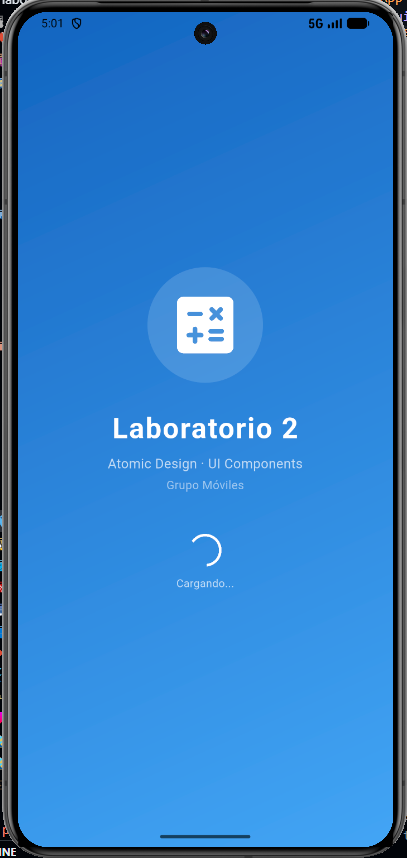
\includegraphics[width=\linewidth]{img/splashStart.png}
  \captionof{anexofloat}{Splash screen -- Pantalla de bienvenida}
\end{minipage}
\hfill
\begin{minipage}[t]{0.45\textwidth}
  \centering
  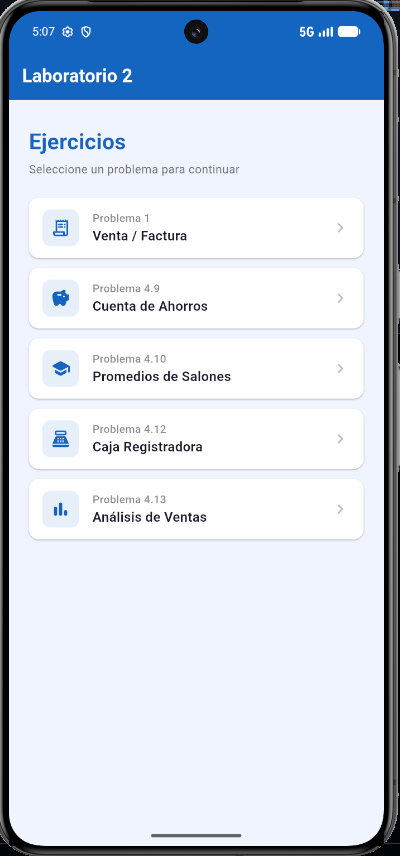
\includegraphics[width=\linewidth]{img/menu.png}
  \captionof{anexofloat}{Menú principal con rutas nombradas}
\end{minipage}

\vspace{1.2cm}

% --- Fila 2 ---
\noindent
\begin{minipage}[t]{0.45\textwidth}
  \centering
  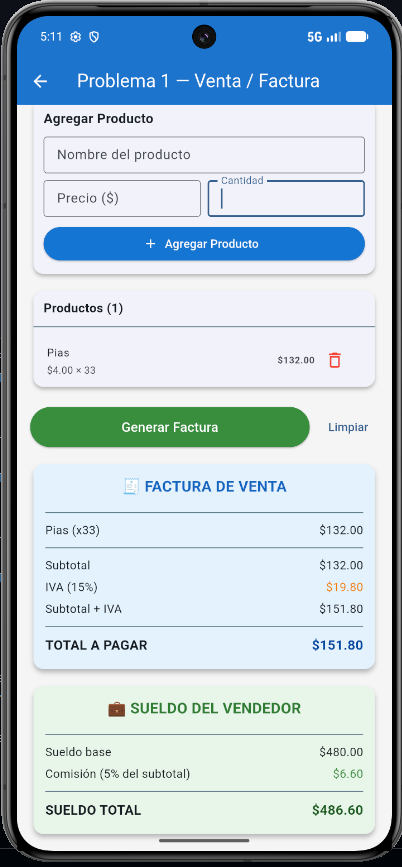
\includegraphics[width=\linewidth]{img/problema1.png}
  \captionof{anexofloat}{Problema 1 -- Venta y Factura}
\end{minipage}
\hfill
\begin{minipage}[t]{0.45\textwidth}
  \centering
  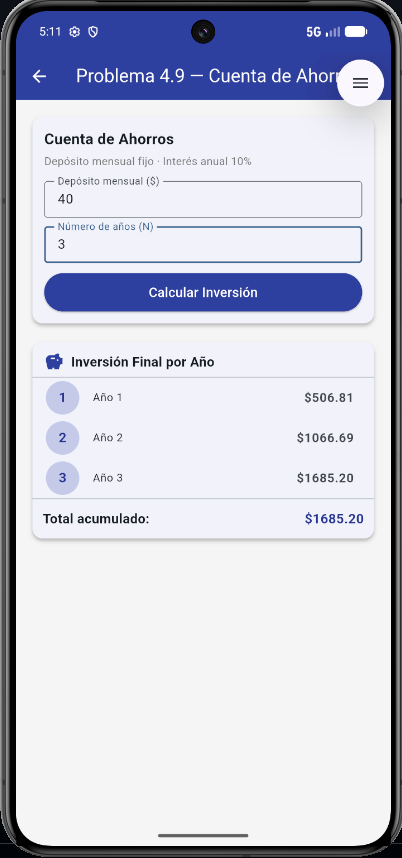
\includegraphics[width=\linewidth]{img/problema4.9.png}
  \captionof{anexofloat}{Problema 4.9 -- Cuenta de Ahorros}
\end{minipage}

\vspace{1.2cm}

% --- Fila 3 ---
\noindent
\begin{minipage}[t]{0.45\textwidth}
  \centering
  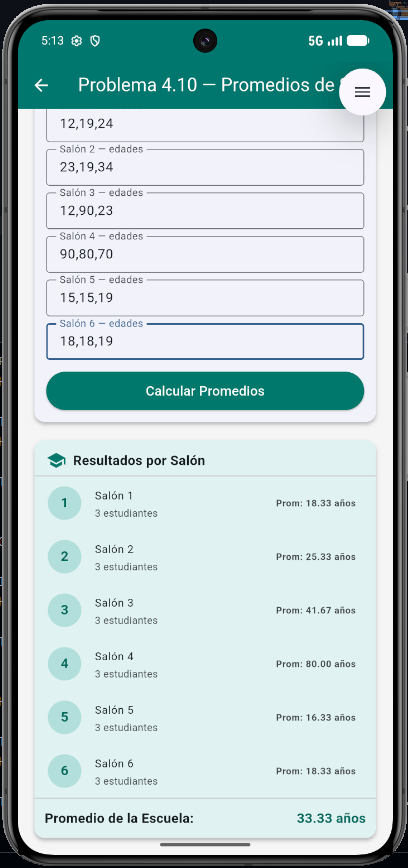
\includegraphics[width=\linewidth]{img/ejercicio4.10.png}
  \captionof{anexofloat}{Problema 4.10 -- Promedios de Salones}
\end{minipage}
\hfill
\begin{minipage}[t]{0.45\textwidth}
  \centering
  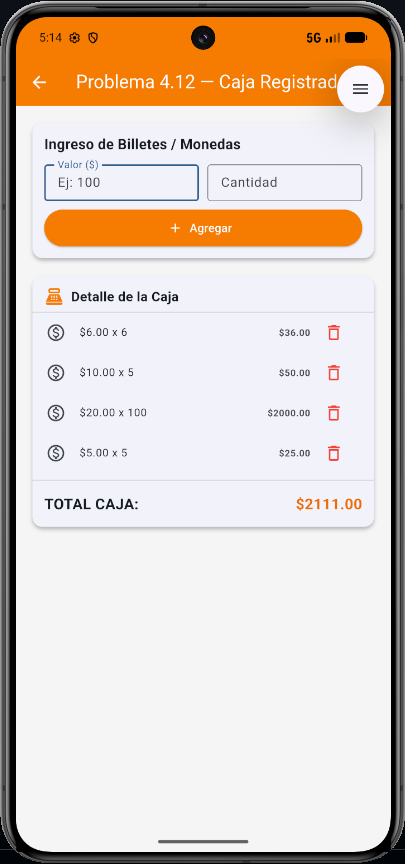
\includegraphics[width=\linewidth]{img/ejercicio4.12.png}
  \captionof{anexofloat}{Problema 4.12 -- Caja Registradora}
\end{minipage}

\vspace{1.2cm}

% --- Fila 4 ---
\noindent
\begin{minipage}[t]{0.45\textwidth}
  \centering
  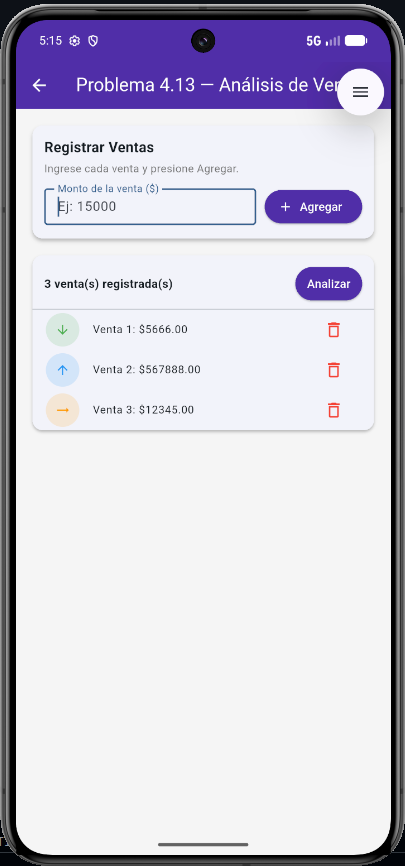
\includegraphics[width=\linewidth]{img/ejercicio4.13.png}
  \captionof{anexofloat}{Problema 4.13 -- Análisis de Ventas}
\end{minipage}

\end{document}
